% hello.tex - Our first LaTeX example!

\documentclass{article}
\usepackage{graphicx}
\usepackage[top=2.54cm, bottom=2.54cm, left=1.25cm, right=1.25cm]{geometry}
\usepackage{mathtools}
\DeclarePairedDelimiter{\abs}{\lvert}{\rvert}
\usepackage{enumerate}
\usepackage{url}


\begin{document}

\title{Foosball: CS296 Project, Group 27}

\author{
Kiran Y - 120050049,\\
\texttt{120050049@iitb.ac.in,}\\
Mihir -12D020007\\
\texttt{mihirk.1994@iitb.ac.in}\\
Harinandan Teja-120050066\\
\texttt{120050066@iitb.ac.in}\\
}
\date{\today}

\maketitle

\section{Introduction}
This report explains in detail the project we created- a foosball table- in Box2d. We describe in brief the bodies,fixtures and constraints we used to create this simulation.\\
Here is the initial model of our simulation:\\
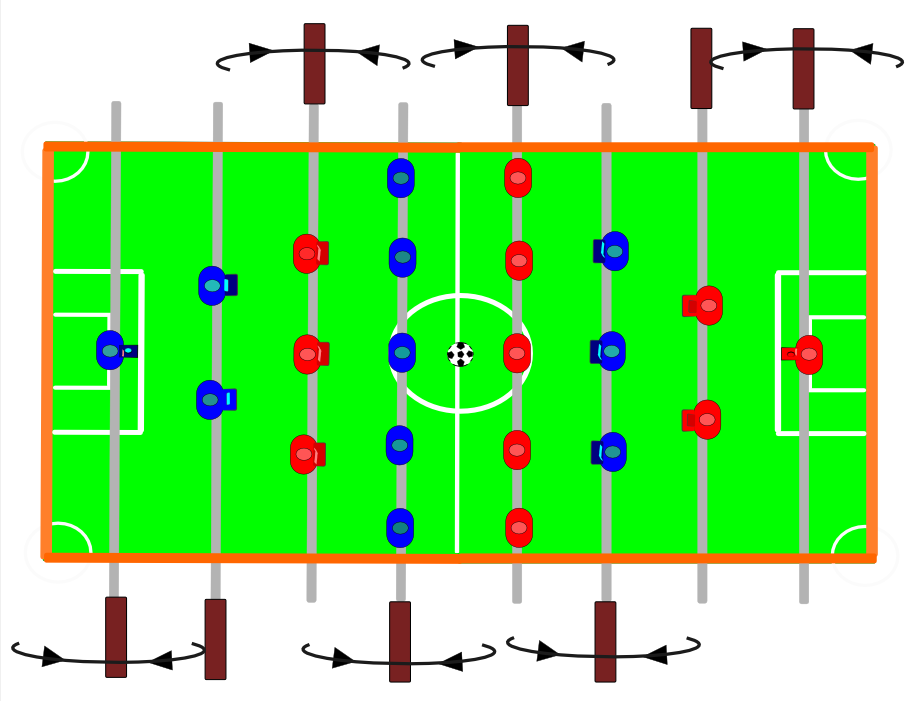
\includegraphics[width=100pt,height=100pt]{foosball}

\section{Design}
We simulated the game of foosball using a bounding table, rods and rigid bodies representing players attached to each rod. Whenever the ball enters one of the goals situated at either end, a score variable is updated and this is shown by moving one of the relevant score blocks present on either side of the table. The first team to seven goals is the winner.\\

The simulation consists of a ball which moves around on the frictionless table colliding with everything it comes in contact with.\\

There are (transparent) rods at relevant locations on the table, constrained to move upto a certain limit in the upward or downward direction. The players attached to each rod can be moved towards either the left or right upto a certain limit. The user also has the option to turn the rod enough to lift all its players off the table.We used the \texttt{b2PrismaticJoint} to simulate motion of these players.\\

The simulation is heavily dependent on user input. We implemented this overloading the \texttt{keyboard()} function of the \texttt{base\_sim\_t} class of Box2D.\\

It was a challenge for us to implement the constraints required by the nature of the game, and we think that usage of prismatic joints and using the \texttt{filter} attributes of Box2D objects to cater to all aspects of motion of the players has made our design more efficient. We also feel that using static objects to constrain the motion of the rods (as explained later) was a simple yet effective feature.\\

\section{Parts of the simulation}

\subsection{Table}
The entire game is played within the confines of the table, which serves to restrict the motion of the ball and rods. This was implemented using four box shapes.\\
%\includegraphics[width=100pt,height=100pt]{Platform}

\subsection{Rods}
Rods are thin dynamic \texttt{Box} objects located at appropriate locations on the table. Two pairs of small static objects are located on either side of the rod at the point where it enters and leaves the table to constrain its motion in the y direction.\\

At any given point, only one rod per team is active. The user can change the active rod by giving a keyboard input.\\

Each rod contains one anchor of a prismatic joint, the other end of which is connected to a Player body.\\

\subsection{Player}
A player is a small,rigid and dynamic body which is attached to a rod via a prismatic joint. All players on the current active rod can be move right or left(upto a certain limit) by a keyboard input.\\

The user can also lift the players of a rod off the table (meaning that the ball can pass underneath them) by pressing the right motion key while the players are at the maximum right position (similarly for the left). This can be viewed as a change in the shape(fixture) of the players.\\

These are implemented by setting appropriate attributes on the prismatic joint and by setting the fixtures and filter bits of the players accordingly.\\
\subsection{Ball}
The ball is a \texttt{b2Circle} shaped \texttt{bullet} object which keeps on moving around and being struck by the players/table walls. Scores are updated when the ball enters either of the goals.\\

\section{Conclusion}
The simulation is identical to the old one for the intial part. When the light box flies up into the air, it knocks the new sphere onto the dominoes and all of them fall down into a new box. The old sphere comes to rest near the wall of the new box. The rest of the animation is unchanged\\
In conclusion, we have added a few features to the simulation to make it more interesting while conserving its basic functionality \\
\bibliographystyle{plain}
\bibliography{cs296_report_27}

\end{document}
